\documentclass[times, 10pt,twocolumn]{article} 
\usepackage{latex8}


\usepackage{graphicx,amsmath,comment,fullpage}
\newcommand{\igH}[1]{\includegraphics[height=.9\textheight]{#1}}
\newcommand{\igW}[1]{\includegraphics[width=.9\textwidth]{#1}}
\newcommand{\igWh}[1]{\includegraphics[width=.7\textwidth]{#1}}
\newcommand{\igWhalf}[1]{\includegraphics[width=.45\textwidth]{#1}}
\newcommand{\lda}{Latent Dirichlet Allocation}


\author{Abram Hindle and Michael Godfrey and Ric Holt \\
\{ahindle,migod,holt\}@cs.uwaterloo.ca\\
Software Architecture Group (SWAG)\\
University of Waterloo\\
}



\title{Windowed Developer Topic Analysis}

\usepackage{rotating}   
\begin{document}


\newcommand{\affaddr}[1]{#1}
\newcommand{\aemail}[1]{#1}
%\numberofauthors{5}
\author{
%\alignauthor
Abram Hindle\\
%\affaddr{David Cheriton School of Computer Science}\\
\affaddr{University of Waterloo}\\
\affaddr{Waterloo, Ontario}\\
\affaddr{Canada}\\
\aemail{ahindle@cs.uwaterloo.ca}
%\alignauthor
\and
Michael W. Godfrey\\
%\affaddr{David Cheriton School of Computer Science}\\
\affaddr{University of Waterloo}\\
\affaddr{Waterloo, Ontario}\\
\affaddr{Canada}\\
\aemail{migod@cs.uwaterloo.ca}
%\alignauthor
\and
Richard C. Holt\\
%\affaddr{David Cheriton School of Computer Science}\\
\affaddr{University of Waterloo}\\
\affaddr{Waterloo, Ontario}\\
\affaddr{Canada}\\
\aemail{holt@cs.uwaterloo.ca}
%\alignauthor
%\and
%Gregorio Robles\\
%\affaddr{GSyc}\\
%\affaddr{Universidad Rey Juan Carlos}\\
%\affaddr{Madrid}\\
%\affaddr{Spain}\\
%\aemail{grex@gsyc.escet.urjc.es}
}






\maketitle
\begin{abstract}

  At different times, developers focus on different topics and tasks
  during development.  These different topics and times of focus might
  be obvious to developers familar with the project, but other
  stakeholders, like managers, might be less aware of the topics of
  development. Imagine the scenario where developers had to deal with
  issues orthogonal to the features suggested, at the end of the
  iteration a manager would wonder where all the time went, the
  developers might have just blocked all sides issues in with features
  they were initially working on, they might not have noticed their
  focus had changed.  Currently it is difficult for stakeholders to
  audit what actually occurred and when certain features or topics
  were focussed on. We propose and provide a visualization of the
  changing development topics over time. Our approach takes a topic
  analysis tool like Latent Dirichlet Allocation (LDA) or Latent
  Semantic Indexing (LSI) and instead of applying the tool to the
  entire corpus we apply to windows of the corpus. This allows us to
  see the unique topics of development occuring during a particular
  time period and then see if these individual topics ever reappear.
  





%   In this lab report we seek to explore how topics shift over time in
%   the source control repository of a project. We analyze commit
%   comments, and even source code per revision per each time window and
%   extract the topics prevelant in that window. We expect that topic
%   sets will change over time and the change in topic sets indicate a
%   change in the focus of development. We suppose this could help us to
%   segment the revisions on the time line to discover parts of an
%   iteration. For topic extraction we use \lda (LDA).

\end{abstract}

\section{Introduction}

%?


% 

% In the presence of fine grained changes and detailed changelogs

% Developers topics the focus of develop

% many changelogs how to sort by change type

% interleaved changes relate similar changes

What happened in the previous iteration? What were the developers
working on? What was the developer in the next cubicle working on?
What were the common topics and issues dealt with in the current
release of the software? What were the topics of the previous release?
Given the requirements agreed to at the start of the iteration did our
developers work on them? What else did they work on. Were there issues
which were orthogonal to the

Topic analysis, with respect to Software Control Systems (SCSs), is
valuable as it has many uses for the stakeholders involved.  Example
scenarios where the usage of these techniques would prove useful are
numerous. Imagine a development team has agreed to implement some
features at the start of an iteration. By the end of the iteration
only some of the agreed upon features are implemented. The developers
swear they were focusing solely on the features agreed upon. Topic
analysis could help by teasing out the distinct topics or focusses of
the developers. Perhaps the developers had to deal with issues
orthogonal to the features they were working on, but were probably
necessary to complete such features. Developers might have grouped
those orthogonal changes into one of the features they were working
on, thus when asked about how their time was spent the orthogonal
changes would not be covered. This is what we hope that windowed topic
analysis can uncover. If windowed topic analysis can discover
important but overlooked topics, it can help both developers and
managers. Developer can reflect and see a good summary of what worked
on, and managers can see the focus of development while still
remaining relatively high level.



We propose to extend common concept analysis techniques by executing
them over windows of documents over time. We hope by looking at topic
clusters over time we can identify continuous effort on a select
group of topics.

Topic analysis of fine-grained revisions is important as often
revisions belonging to different topics are interleaved or even mixed
inside of commits.  Sometimes a single revision to a file contains
multiple bug fixes.  Using powerful topic analysis techniques like
Latent Semantic Indexing (LSI) or Latent Dirichlet Allocation (LDA)
one can seperate these mixed signals into coherent topics. In this
case a topic is a set of tokens that are related to each other.

% We suppose this could help us to segment the revisions on the time
% line to discover parts of an iteration.

Another use of topic analysis is to help us partition a project's
time-line into sub-iterations of developer focus. By breaking apart an
iteration we might be able to extract the underlying software
development process from these artifacts or at the very least what
maintenance was occurring in the repository at that time.

In this paper we seek to explore how topics shift over time in the
source control repository of a project. We analyze commit comments per
revision in each time window and we extract the topics in that time
window. We expect that topics in each window will change over time and
the similarities and differences in these sets of topics will indicate
both developer focus and changes in developer focus.

Our contributions include:
\begin{itemize}
\item Demonstrating the value of windowed topic analysis
\item Multiple visualizations of trends over time
\end{itemize}


\section{Background}


Some terms we will be using for the rest of the paper include:
message, word distribution, topic and trend. Messages are block of
text written by developers, in this paper messages will be the CVS
commit comments. Word distributions are the summary of a message by
word count, effectively the word distribution will be over all
messages looked at but since most words will not appear in a message,
a word distribution is effectively a word count divided by the message
size. A topic is a unique word distribution, but effectively a set of
words unique to an independant behaviour in the text corpus, in this
paper we often summarize topics by their top 10 more frequent words.
A trend is a one or more similar topics which reoccur over
time. Trends are important because they are sets of topics which
reoccur over the development of a project.


%\subsection{Intro to LDA}

%XXX explain LDA \cite{944937}

Latent Dirichlet Alloation (LDA)~\cite{944937} is a competitor to
Latent Semantic Indexing (LSI), probabilistic Latent Semantic Indexing
(pLSI) and semantic clustering. It is used for document modelling,
document clustering and collaborative filtering. What LDA attempts to
do is model a documents as mixture model of topics.  The common use of
LDA in software engineering
literature~\cite{lukins2008,10.1109/MSR.2007.20,NIPS2007637,1321709}
is to extract topic clusters from documents such as methods, bug
reports, source code and files.

Our blackbox view of LDA and LSI is that they extract topic clusters
from the documents that are independant from one another. LDA doesn't
name these clusters but the clusters consist of words whose
relationship is often obvious to someone familar with the
corpus. Technically we could swap LDA for LSI. Our data is posed as
documents with word distributions (word counts per documents) and LDA
extracts distinct topics (clusters of words) from the documents.

\subsection{LDA, LSI and Semantic Clustering}

Linstead et al has proposed an author source code model using
LDA~\cite{10.1109/MSR.2007.20,NIPS2007637,1321709}. They used an
author-topic (AT) model~\cite{1036902} to infer the association or
expertise of a particular developer with a particular code topic
extracted from the source control system.

Lukins, Kraft and Etzkorn~\cite{lukins2008} use LDA to help query for
finding related documents during bug localization tasks. They used LDA
to build a topic model and then query against it using sample
documents, the query would the proportion of topics that were
associated with the query and thus the related documents.

LSI is related to LDA and has been used to identify topics in software
artifacts for forumal concept analysis and concept
location~\cite{1421013,1374321,10.1109/ICPC.2007.13,10.1109/ICPC.2006.17}.
This is when concepts are automatically extracted from source code or
documents are related to part of the source code.  Concept location is
how high level concepts relate to low level entities like source code,
for instance when fixing a bug how do the concepts in the bug report
map back to the source code?  Semantic Clustering has also been used
for similar reason~\cite{1698774,1566153}.

Grant et al.~\cite{scottcordy} have used an alternative technique to
LSI and LDA, they used Independant Component Analysis to seperate
topic signals from software code.

Our technique differs in the sense we apply LDA temporally and we
apply to change comments.

%      1. [ ] LDA itself
%      2. [ ] Maletic stuff
%      3. [ ] WCRE: Scott/Jim
%      4. [ ] WCRE: Bug LDA stuff
%      5. [ ] MSR: Challenge work
%      6. [ ] FCA work
%4. [ ] Methodology [0/9]


\section{First Impressions}

In our first exploratory pass we wanted to see 

Looking at 30 day non-overlapping windows of revisions for MySQL 3.23
(20 topics, top 10 words per topic) we found there were common words
across topic clusters such as diffs, annotate and history. There were
notable transitional topics such as in the first window the word
``bitkeeper'' appears (probably when they adopted Bitkeeper for their
source control system) yet in the following windows there were no
mentions of Bitkeeper. ``RENAME'' also only appeared once in the first
window and never again.

A subsampling of the notable topic words is displayed in Table
\ref{tab:portability}. We tracked one topic cluster which seemed
related to portability. We picked out terms which seem to summarize
those topics.

%Often words are shared across topics, see table \ref{tab:portability}
%for tracking topics about portability.

After viewing these topic is was obvious that we would have to combine
try to track the evolution of topics over the windows or rank topics
by similarity.

%It is apparent that we have to compare these topics some how by
%itemset or similarity.

\begin{table*}
\centering
\begin{tabular}{|ccc|l|}
\hline
2000 &  Jul &  31 &    chmod \\
2000 &  Sep &  29 &    fixes benchmark logging windows \\
2000 &  Nov &  28 &    typo fix insert\_multi\_value \\
2001 &  Jan &  27 &    fixes Innobase Cleanups auto-union \\
2001 &  Mar &  28 &    2 topics bugfix, logging , TEMPORARY,  \\
\hline
2001 &  Jul &  26 &    update Allow TABLES LOCK [a] \\ 

2001 &  Aug &  25 &    tables row version [a] \\
\hline
2001 &  Sep &  24 &    update checksum merge \\
2001 &  Oct &  24 &    fixed fix \\
2001 &  Dec &  23 &    HPUX SCO fix \\
\hline
2002 &  Feb &  21 &    net buffer length  max\_allowed\_packet [b] \\
2002 &  Mar &  23 &    small buf fix [b]  \\
\hline
2002 &  May &  22 &    [popular] fix SCO OSF1 table\_name \\
2002 &  Nov &  18 &    HPUX11 compiler HP \\
\hline
2003 &  Feb &  16 &    Linux errno  [c] \\
2003 &  Mar &  18 &    alarm bookmark bug [c] \\
\hline
2003 &  Sep &  14 &    Auto logging merge windows distribution fix 64-bit 4.0 Cleanup \\
\hline
\end{tabular}
\caption{Tracking topics associated with the word portability, note some continuous blocks}
\label{tab:portability}
\end{table*}

\begin{figure*}
  \centering
  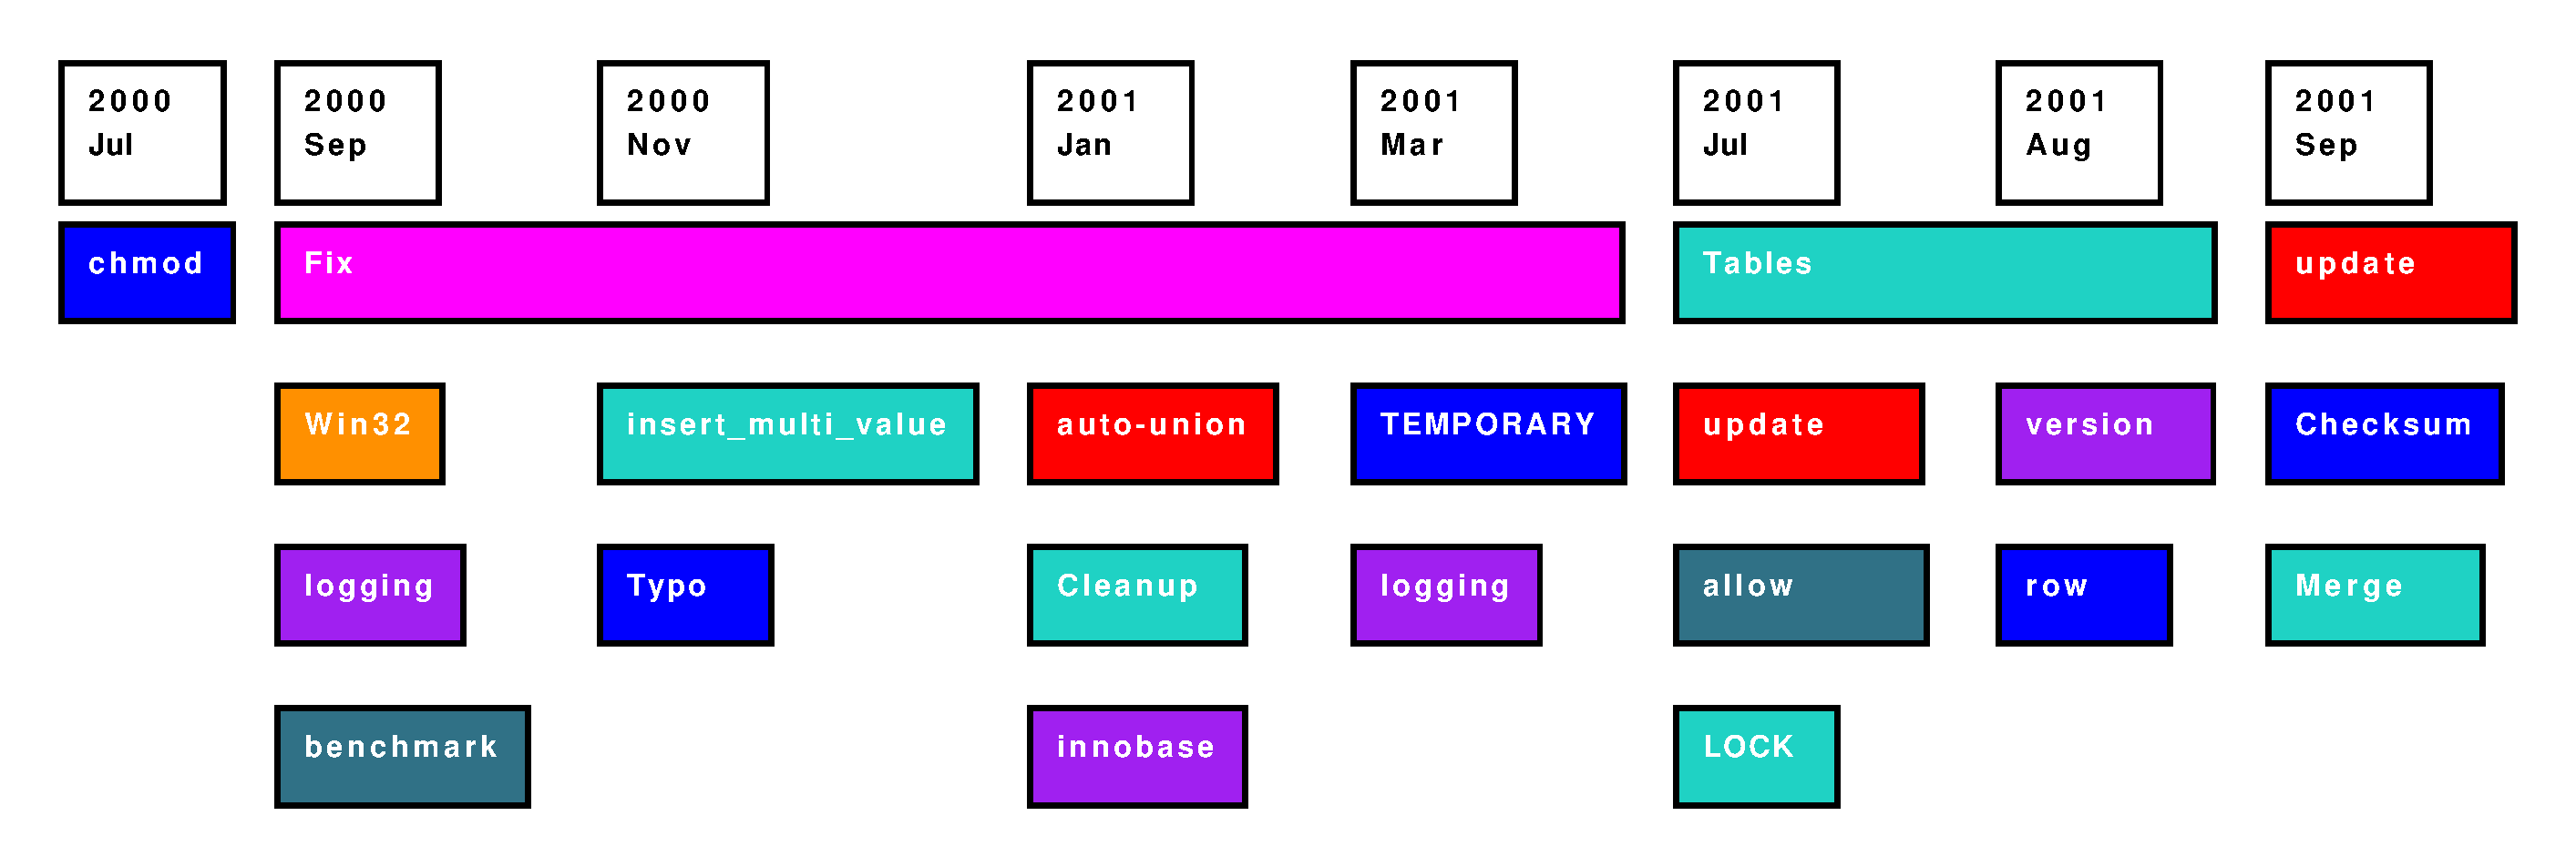
\includegraphics[width=0.9\textwidth]{lda}
  \caption{Example of topics extracted from MySQL 3.23. This is the kind of plot we eventually want to produce: named topics and topic trends}
  \label{fig:lda}
\end{figure*}



\section{Methodology}
\begin{figure*}
  \centering
  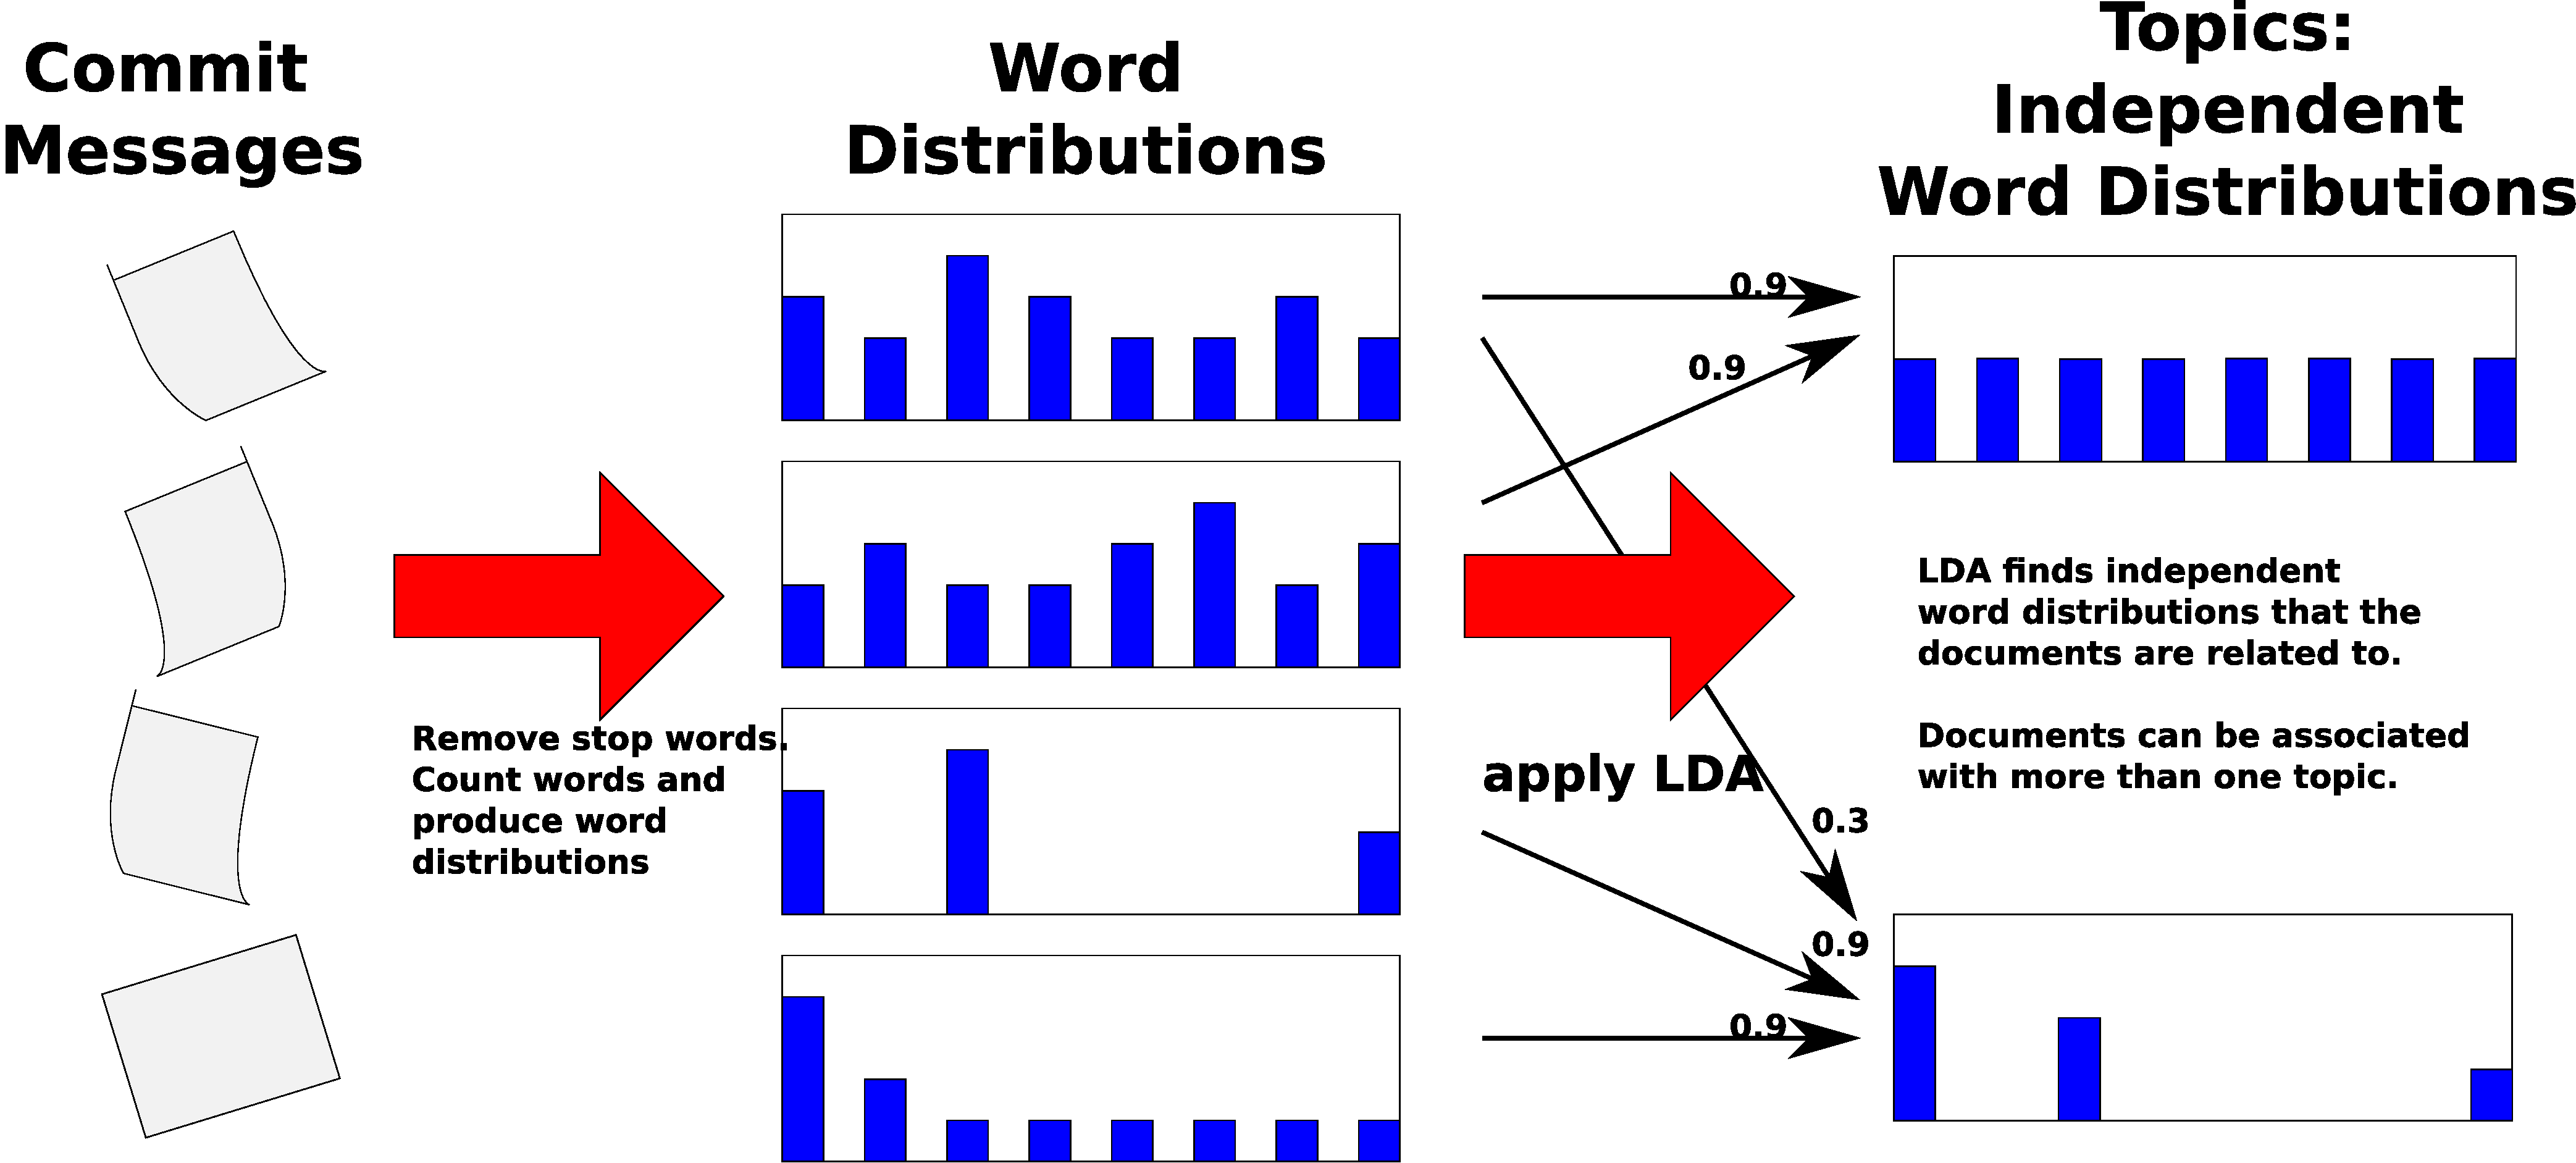
\includegraphics[width=0.9\textwidth]{commit-to-topics} 
  \caption{How commits are analyzed and aggregated into Topics and Trends}
  \label{fig:commits}
\end{figure*}



\subsection{Extract Repos}

We extracted the repositories with software such as rsync, CVSSuck,
\texttt{softChange} and bt2csv.  \texttt{softChange} provided a
general schema for storing revisions. CVSSuck and rsync mirrored CVS
repositories while bt2csv mirrored web accessible bitkeeper
repositories.


%   2. [ ] Extract Documents
\subsection{Extract Documents}
%   3. [ ] Windowed Sets

The document we are analyzing are the changelog comments, these are
the comments added when a revision to the source code is committed.
Documents are converted into word count distributions. These
distributions are can be normalized by by the size of the
message. After all messages are processes the distributions are
extended to include all words in all distributions (each distribution
is extended with word bins of count 0).

\subsection{Windowed Sets}

Given all messages, we group the messages into windows. We could use
overlapping windows, but in this paper we use non-overlapping windows
of a set time unit.  Windowing by time allows for many levels of
granularity. We usually used one month as the length of our time
windows, while we could use different granularities for the study we
think that a month is a sizable unit of development (4 weeks of
development).


\subsection{Apply Topic Analysis to each Window}

Once we have our data windowed, we apply our Topic Analysis tool to
each window and extract the top $N$ topic clusters, we used $20$
topics in our case study. Our Topic Analysis tool is an implementation
of LDA, but we could've used other similar tools like LSI.

This is a very slow step as LDA takes a long time to run, and takes
even longer since we run it once per window.



%\subsection{Extract Clusters}


%   6. [ ] Cluster Similarity [0/1]
\subsection{Cluster Similarity}
%      1. [ ] need the tool
%             grab from the cluster analysis
%   7. [ ] Continuous Cluster Analysis


Once we have our topics extracted for each window , we analyze them
and look for repeating topics. We do this by taking the top 10 most
common words and then comparing them. 

We then abstract these topics by comparing them to each other.  Each
topic is compared to each other topic in the system, given a certain
threshold of top 10 similarity, like 8/10 words. Then given this topic
similarity matrix, we find the transitive closure of similar topics,
that is we fill flood along the similarity arcs until we have
partitioned the topics into clusters of similar topics.  These
clusters of topics are called trends. A trend is probably interesting
and valuable if there is more than 1 topic in the trend.

This technique has weaknesses in that nodes a few neighbors away in
similarity might not share any similar words.  We do this because we
want to be able to color or highlight topics which are related to each
other and track them throughout time.

Once we have determined our similarity clusters we can choose to
analyze and to plot the topics.

\begin{comment}
Topic Clustering
 · Need to track continuous topics across
 · Similarity between topics
 · Clusters of the transitive closure of topics with X%
   similarity
    ­ Fill flood along similarity, make subsets of
      everyone who X% similar to any of their neighbors,
      make that a cluster
\end{comment}

\begin{figure}
  \centering
  \includegraphics[width=0.45\textwidth]{transitiveclosure}
  \caption{Clusting topics by the transitive closure of topic similarity. Nodes are topics and arcs imply similarity}
\label{fig:closure}
\end{figure}



\subsection{Visualization}
%       1. [ ] need the visualizer

We have come up with multiple ways to visualize these topics and
trends.  For all of these plots if we trends which have continuous
segments we plot those segments as joined across time.  We have a
compressed stacked trend view, which displays trends arbitrarily
across the y axis but are placed where they occur on the time-based x
axis. Another plot we have is the trend-time plot, a each trend gets
it own distinct-y value , while the x-axis is time; these topics are
then each plotted on their own line across time as they occur. The
last plot we have is the histogram plot, where we plot each trend on
its own line but stack up the segments of the trend, much like a plot
of counts or a histogram.


The first visualization is a compressed view, we try to sink the
larger trends to the bottom, once the larger trends are stacked, we
fill in the gaps with the smaller trends in the same window and then
stack the smaller trends on top. Although there is a chance that gaps
will be left due to nonoptimal stacking in practice there are lot of
small trends (90\% of all trends contain 1 topic) which fill in these
gaps quickly. The trend segments that share the same color are the
same trend, colors are randomly chosen for each trend, so color
similarity is meaningless, only exact color matching matters.
The compressed view is nice because it shows all of the
information and the repeating continuous trends are easy to pick out,
unfortunately repeating discontinuous trends are harder to spot.

The second visualization is the trend-time plot, it displays repeating
trends more clearly by dedicating a horizonal line for trend segments
dedicated to one trend. This means that if a trend contains
discontinuous segments the segments appear on the same line. One down
side to this view is the least common trends need to be pruned
otherwise it'd take too many horizontal lines to plot them.

The 3rd visualization is the histogram plot which is a lot like the
time-trend plot except the trends are plotted together by stacking to
their row so time information is lost and the trends are ordered by
the number of topics in the trend. The histogram plot shows the count
of instances of a trend and thus indicates which trends occur the
most. Unfortunately due to the large number of topics given allotted
space it is often best to crop off the trends with only one topic,
otherwise the tail is long.

\begin{figure*}
  \centering
  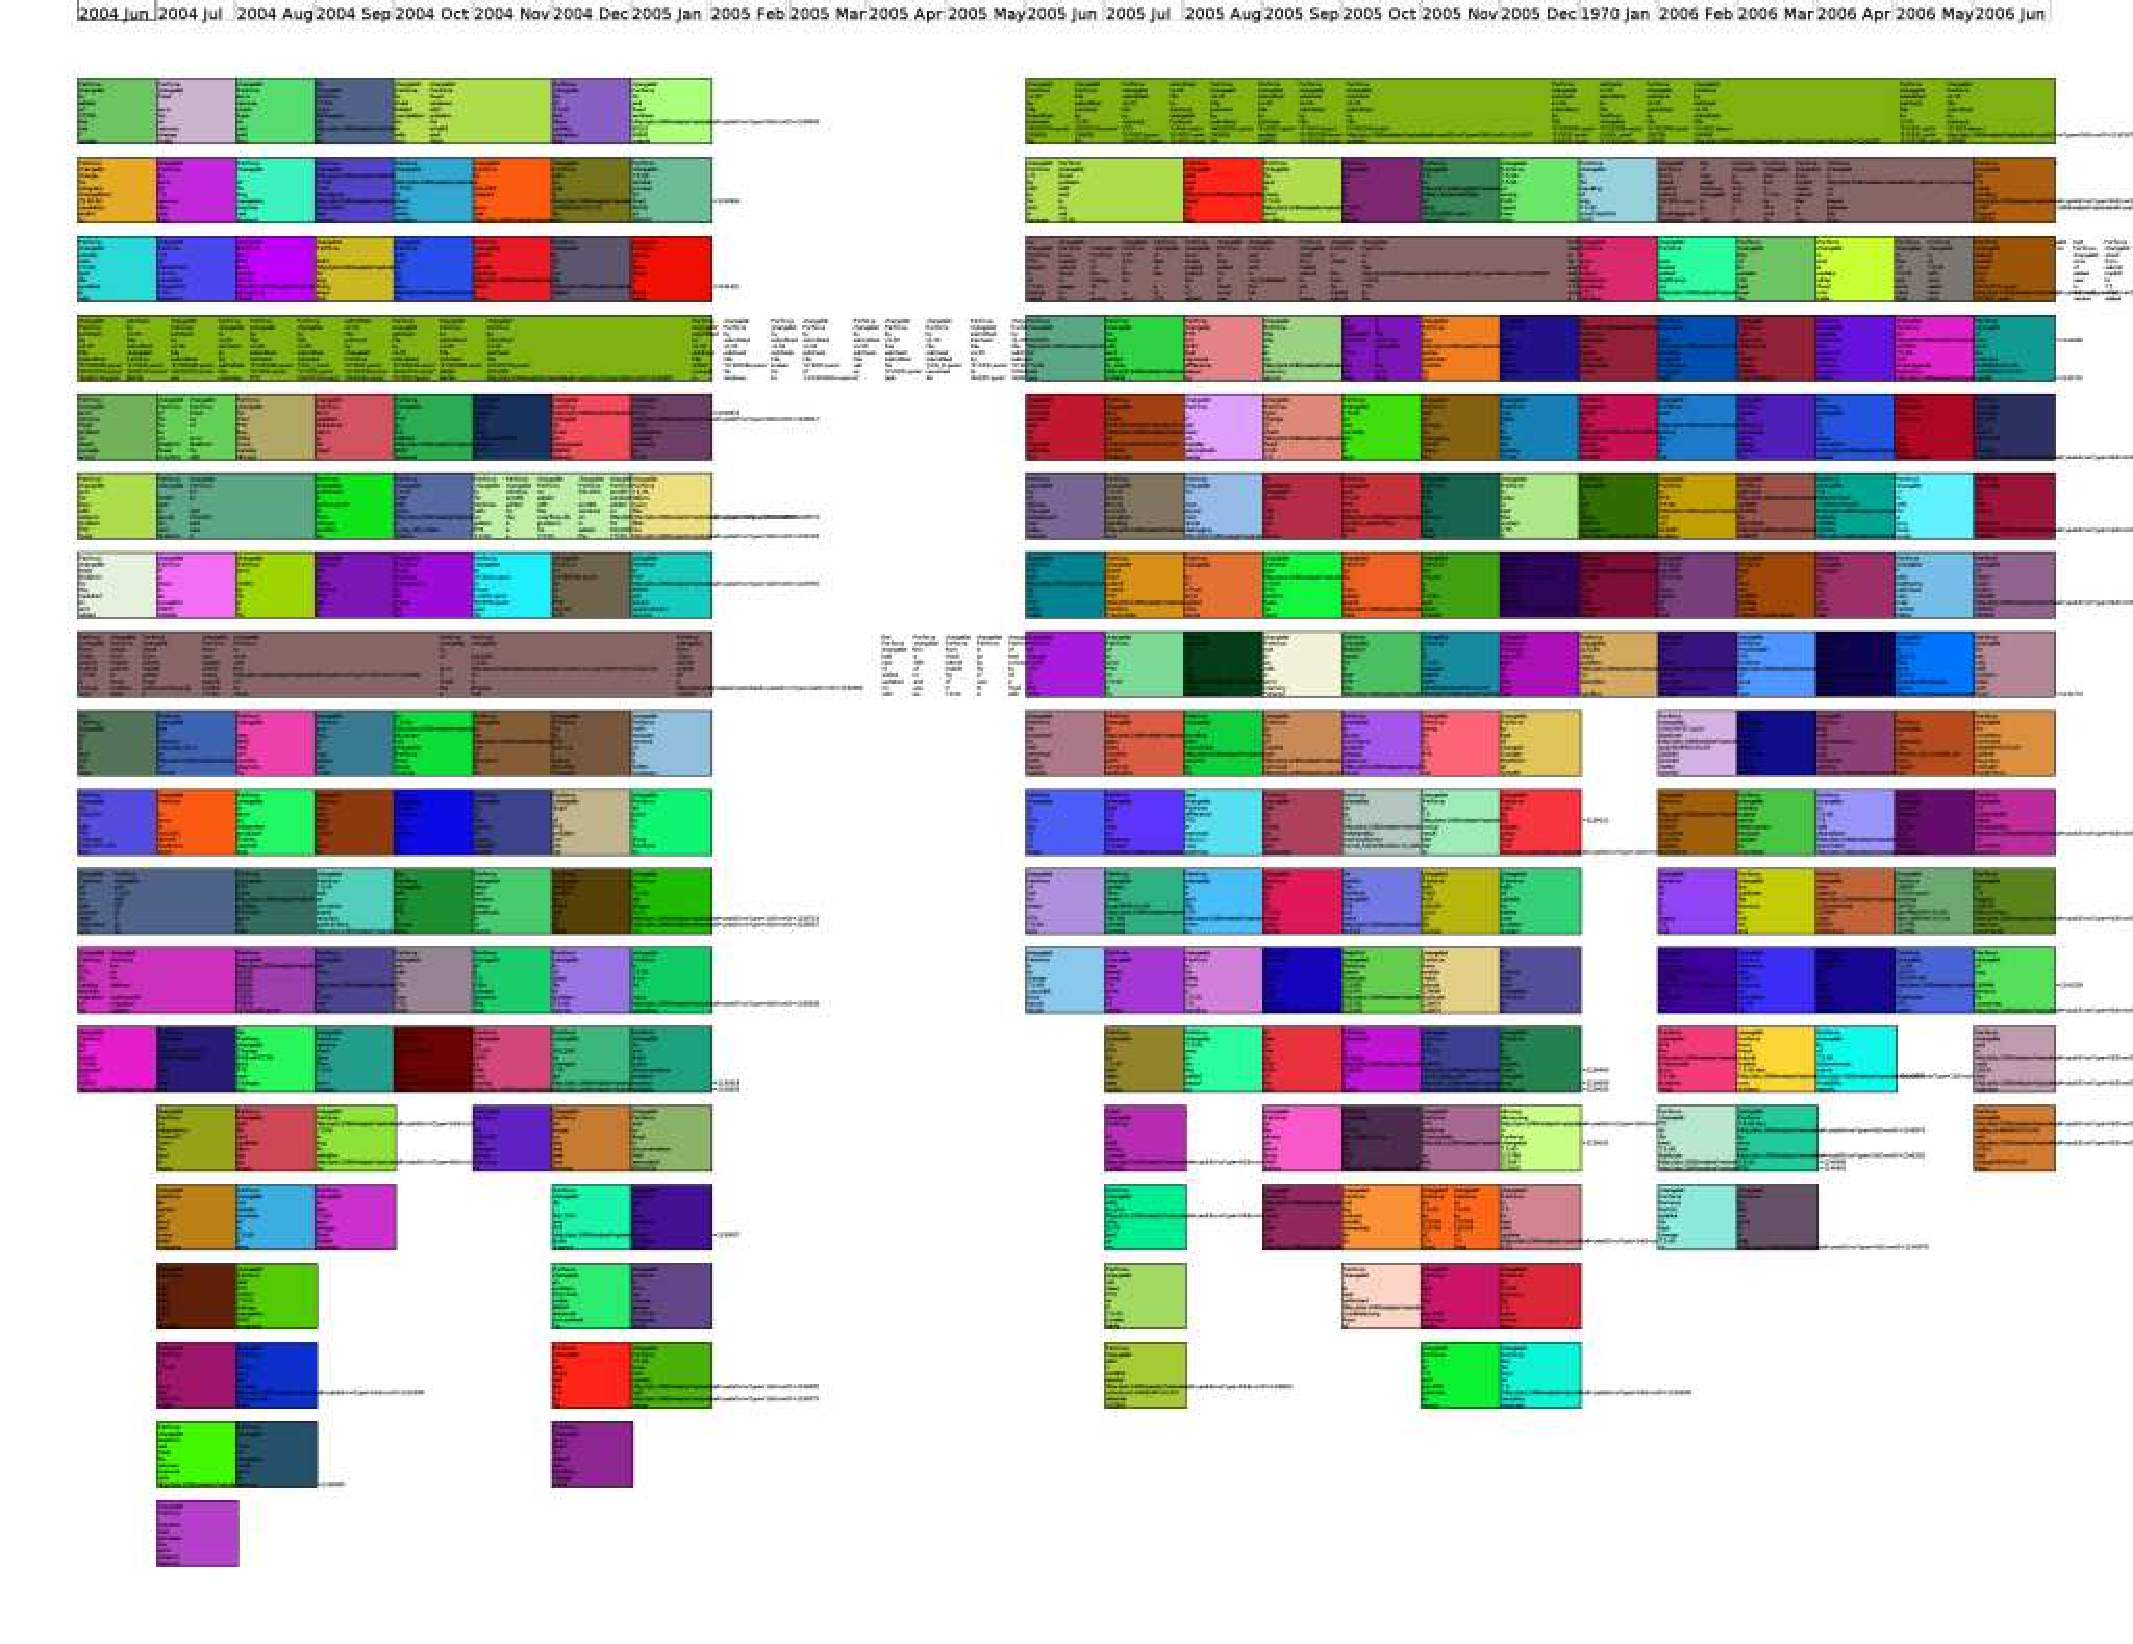
\includegraphics[width=1.0\textwidth]{fixed-time-smear-plot-scaled}
  \caption{Compact Trend Plot Topics per Month for MaxDB 7.500}
  \label{fig:topicsmear}
\end{figure*}


\begin{figure}
  \centering
  \includegraphics[width=0.45\textwidth]{fixed-time-smear-plot-cropped}
  \caption{Zoomed in Slice Compact Trend Plot of Topics per Month for MaxDB 7.500}
  \label{fig:zoomedsmear}
\end{figure}


\begin{figure}
  \centering
  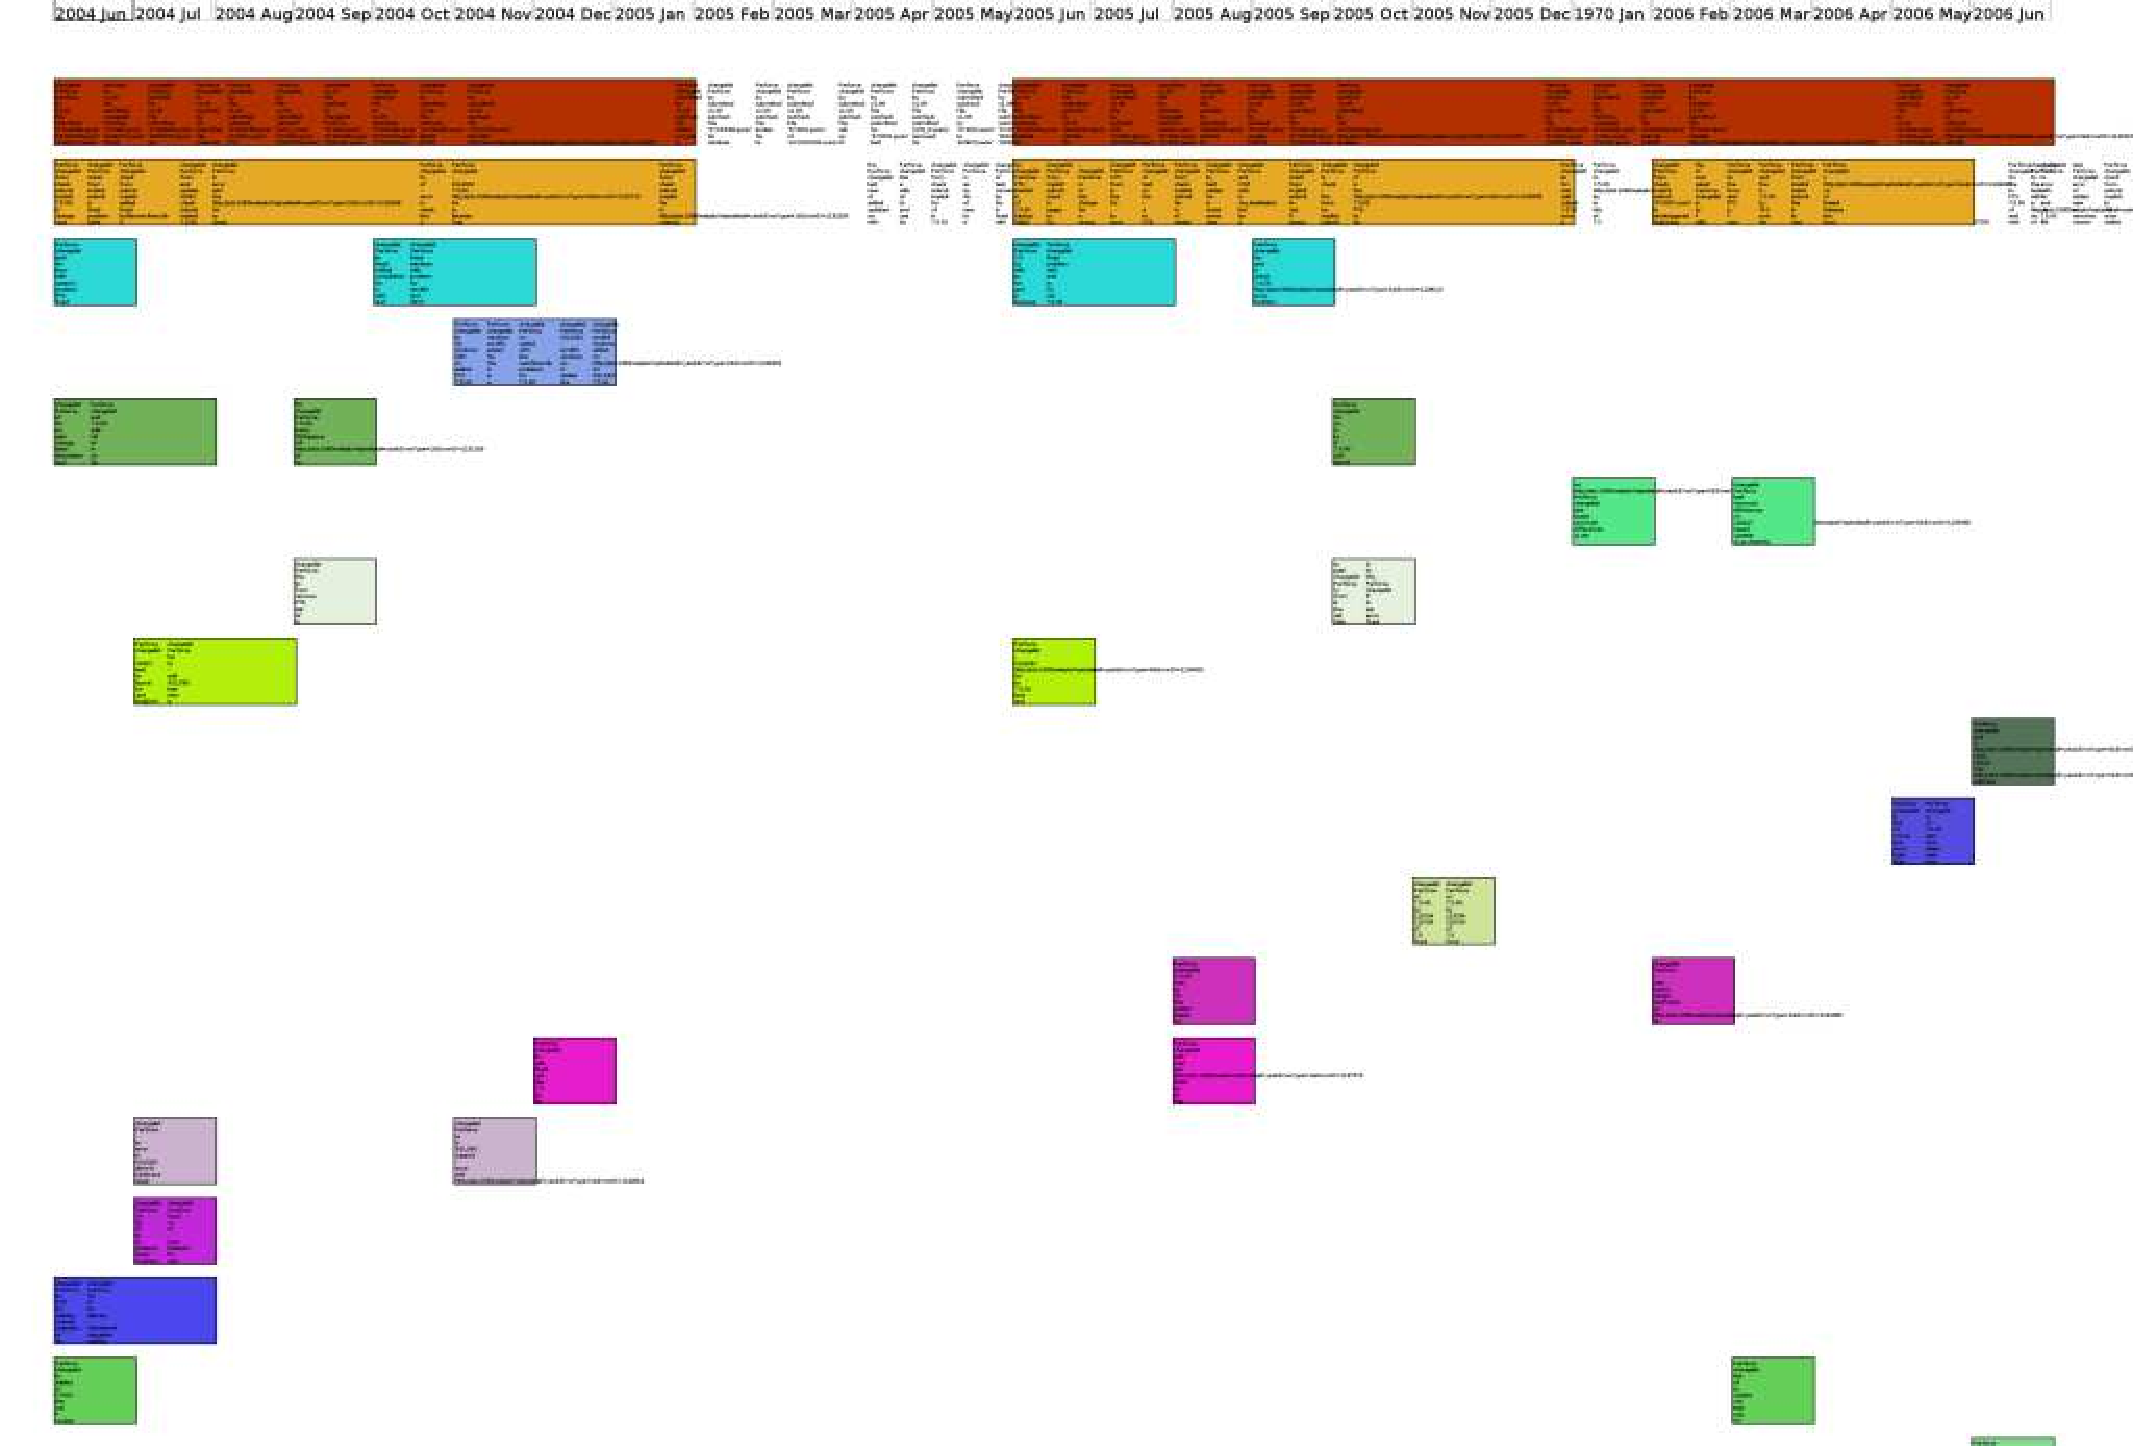
\includegraphics[width=0.45\textwidth]{class-smear-plot-crop-scaled}
  \caption{Trend Time Line: Trends plotted over time of MaxDB 7.500}         
  \label{fig:trendtimeline}
\end{figure}


\begin{figure}
  \centering
  \includegraphics[width=0.45\textwidth]{histogram-cropped-scaled}
  \caption{Top part of trend histogram, ordered by topic occurance for MaxDB 7.500}       
  \label{fig:histogram}
\end{figure}


\subsection{Datasets and Tools}

To extract data from CVS and BitKeeper we used softChange to extract
CVS repositories and provide a schema for our revision data. We used
bt2csv to extract BitKeeper revisions from BitKeeper web repositories.

We extracted the repositories of: PostGreSQL, MaxDB and
Firebird.

% Extractors:
% \begin{itemize}
% \item CVSSuck - CVS Suck mirrors RCS files from a CVS repository. 
% \item softChange - extract CVS facts to a PostgreSQL database.
% \item bt2csv - Convert BitKeeper repositories to facts in CSV
%   databases.
% \end{itemize}

Our analysis tools consisted of: Hiraldo-Grok, an OCaml based spin off
of Grok used for answering queries; Gnuplot, a graph plotting package;
lda-c, a LDA package implemented by Biel; and our topic plotter,
implemented in Haskell.


%   1. [ ] LDA

%   2. [ ] Extractor

%   3.   Similarity

%   4.   Smearing

%   5.   Visualizer




%LDA Skeleton
%1. [ ] Abstract 
%2. [ ] Introduction

%3. [ ] Previous Work [0/2]
%   2. [ ] LDA Work [0/6]




\section{Results}

We applied our tools and visualizations to the repositories of
multiple database systems. 

%   1. Interesting smears 
%   2.   postgresql
\subsection{Postgresql}
%   3.   mysql

PostgreSQL did not have many trends with two or more topics, but it
did have one large mega-trend which stretched across most of its
existence. Much of the mega-trend consisted of stop words but it did
include topics which had words such as patch, fix, update.

The second largest topic was interesting because it dealt changes from
1998, from developers using Central Europe Time (CEST), the two
notable tokens were 1998 and CEST. These changes seem to be patches
submitted by one particular developer who used that timezone.

The third largest trend seemed to be about copying and moving files
between branches as it referenced the old branch. This is a side
effect of the programmers manually recording such a merge across
branches because CVS cannot.

Once stop words were removed the some of hte purposes became more
clear. The mega trend disappeared, the largest trend became bug fixes
submitted by Dal Zotto which is a short trend.


% Large Trends is not the point!!!
% That's what normal LDA gives us

But large trends are not the point, by investigating windowed trends
we want more local information about trends being worked on.

\subsection{Firebird}
%   5.   what's that other db?

%XXX needs results

We tracked Firebird from August 2000 to January 2006.
Our first attempt with Firebird resulted in a set of trends that were
dominated by one large trend containing tokens which were mostly stop
words such as ``the to a for of is it'' and references to one author
\texttt{carlosga05}. 

The second largest trend related to branching and possibly merging, it
contained language such as ``was added on branch'' and contained
references to tags and branches.

The third largest trend contained reference to the changelog, the
build system, architecture and platform support. It specifically
mentioned tokens such as ``Solaris port x86''.

Other trends included topics regarding AIX PPC compilation, updating
the build process, internationalization and UTF8, Darwin build support
and bug fixing.

Topics that were not trends that were interesting were external bug
fixes submitted to the project, the developers would write thank yous
in their changelog comments: ``thanks Bill Lam''. Other interesting
topics include tokens and topics such as: ``compiler workarounds'', ``nightly updates'', packets and MSVC++, 

\subsection{MaxDB 7.500}

The plots we produced of MaxDB 7.500 were interesting, there was a
period where no real development occured and thus there were no topics or trends
whatsoever. We have two periods to evaluate for MaxDB 7.500, the first
period from June 2004 to jan 2005, and the second period from June
2005 to June 2006.

The largest common trend has references to build system files like
SYSDD.punix and MONITOR.punix etc. Other tokens mentioned are Sutcheck
v1.09, the prefix SUT stands for Storable Unit Type. Sutcheck would
also automate perforce check-ins.

The second largest common trend seems to be a side effect of an
automated checkin which is annotated as ``implicit checkin''. These
were checkins that were produced when importing changes from an
external Perforce repository.

The third most common trend, seen on Figure \ref{fig:trend}, seemed to
include tokens related to operating system support, such as Linux and
Windows, as well as architecture support, AMD64 and Opteron. The word
problem was common among all of those trends. This trend seemed
related to the smaller fourth largest trend which occurred nearby it
that had AMD64 and Windows tokens.

\subsection{Compare to topics over entire development}

The previous work which leverage LSI or LDA usually extracted a
certain number of topics and tracked them over time. This meant a
static set of topics was tracked across the whole development history
of a project. Thus we really had 20 trends. 

We attempted the same kind of analysis, as shown in
Figure~\ref{fig:statictopics} we extracted 20 topics and then plotted
the number of messages per month which related to that topic. What we
found was that often one topic would dominate the results, while
messages related to other topics didn't appear that often.

This technique seems useful if the 20 extracted topics are relevant
and useful, that said one weakness of this approach is that documents
for a topic might only occur in one time window, yet we're tracking
messages that could be related to it over the entire lifetime of the
project.

\begin{figure}
  \centering
  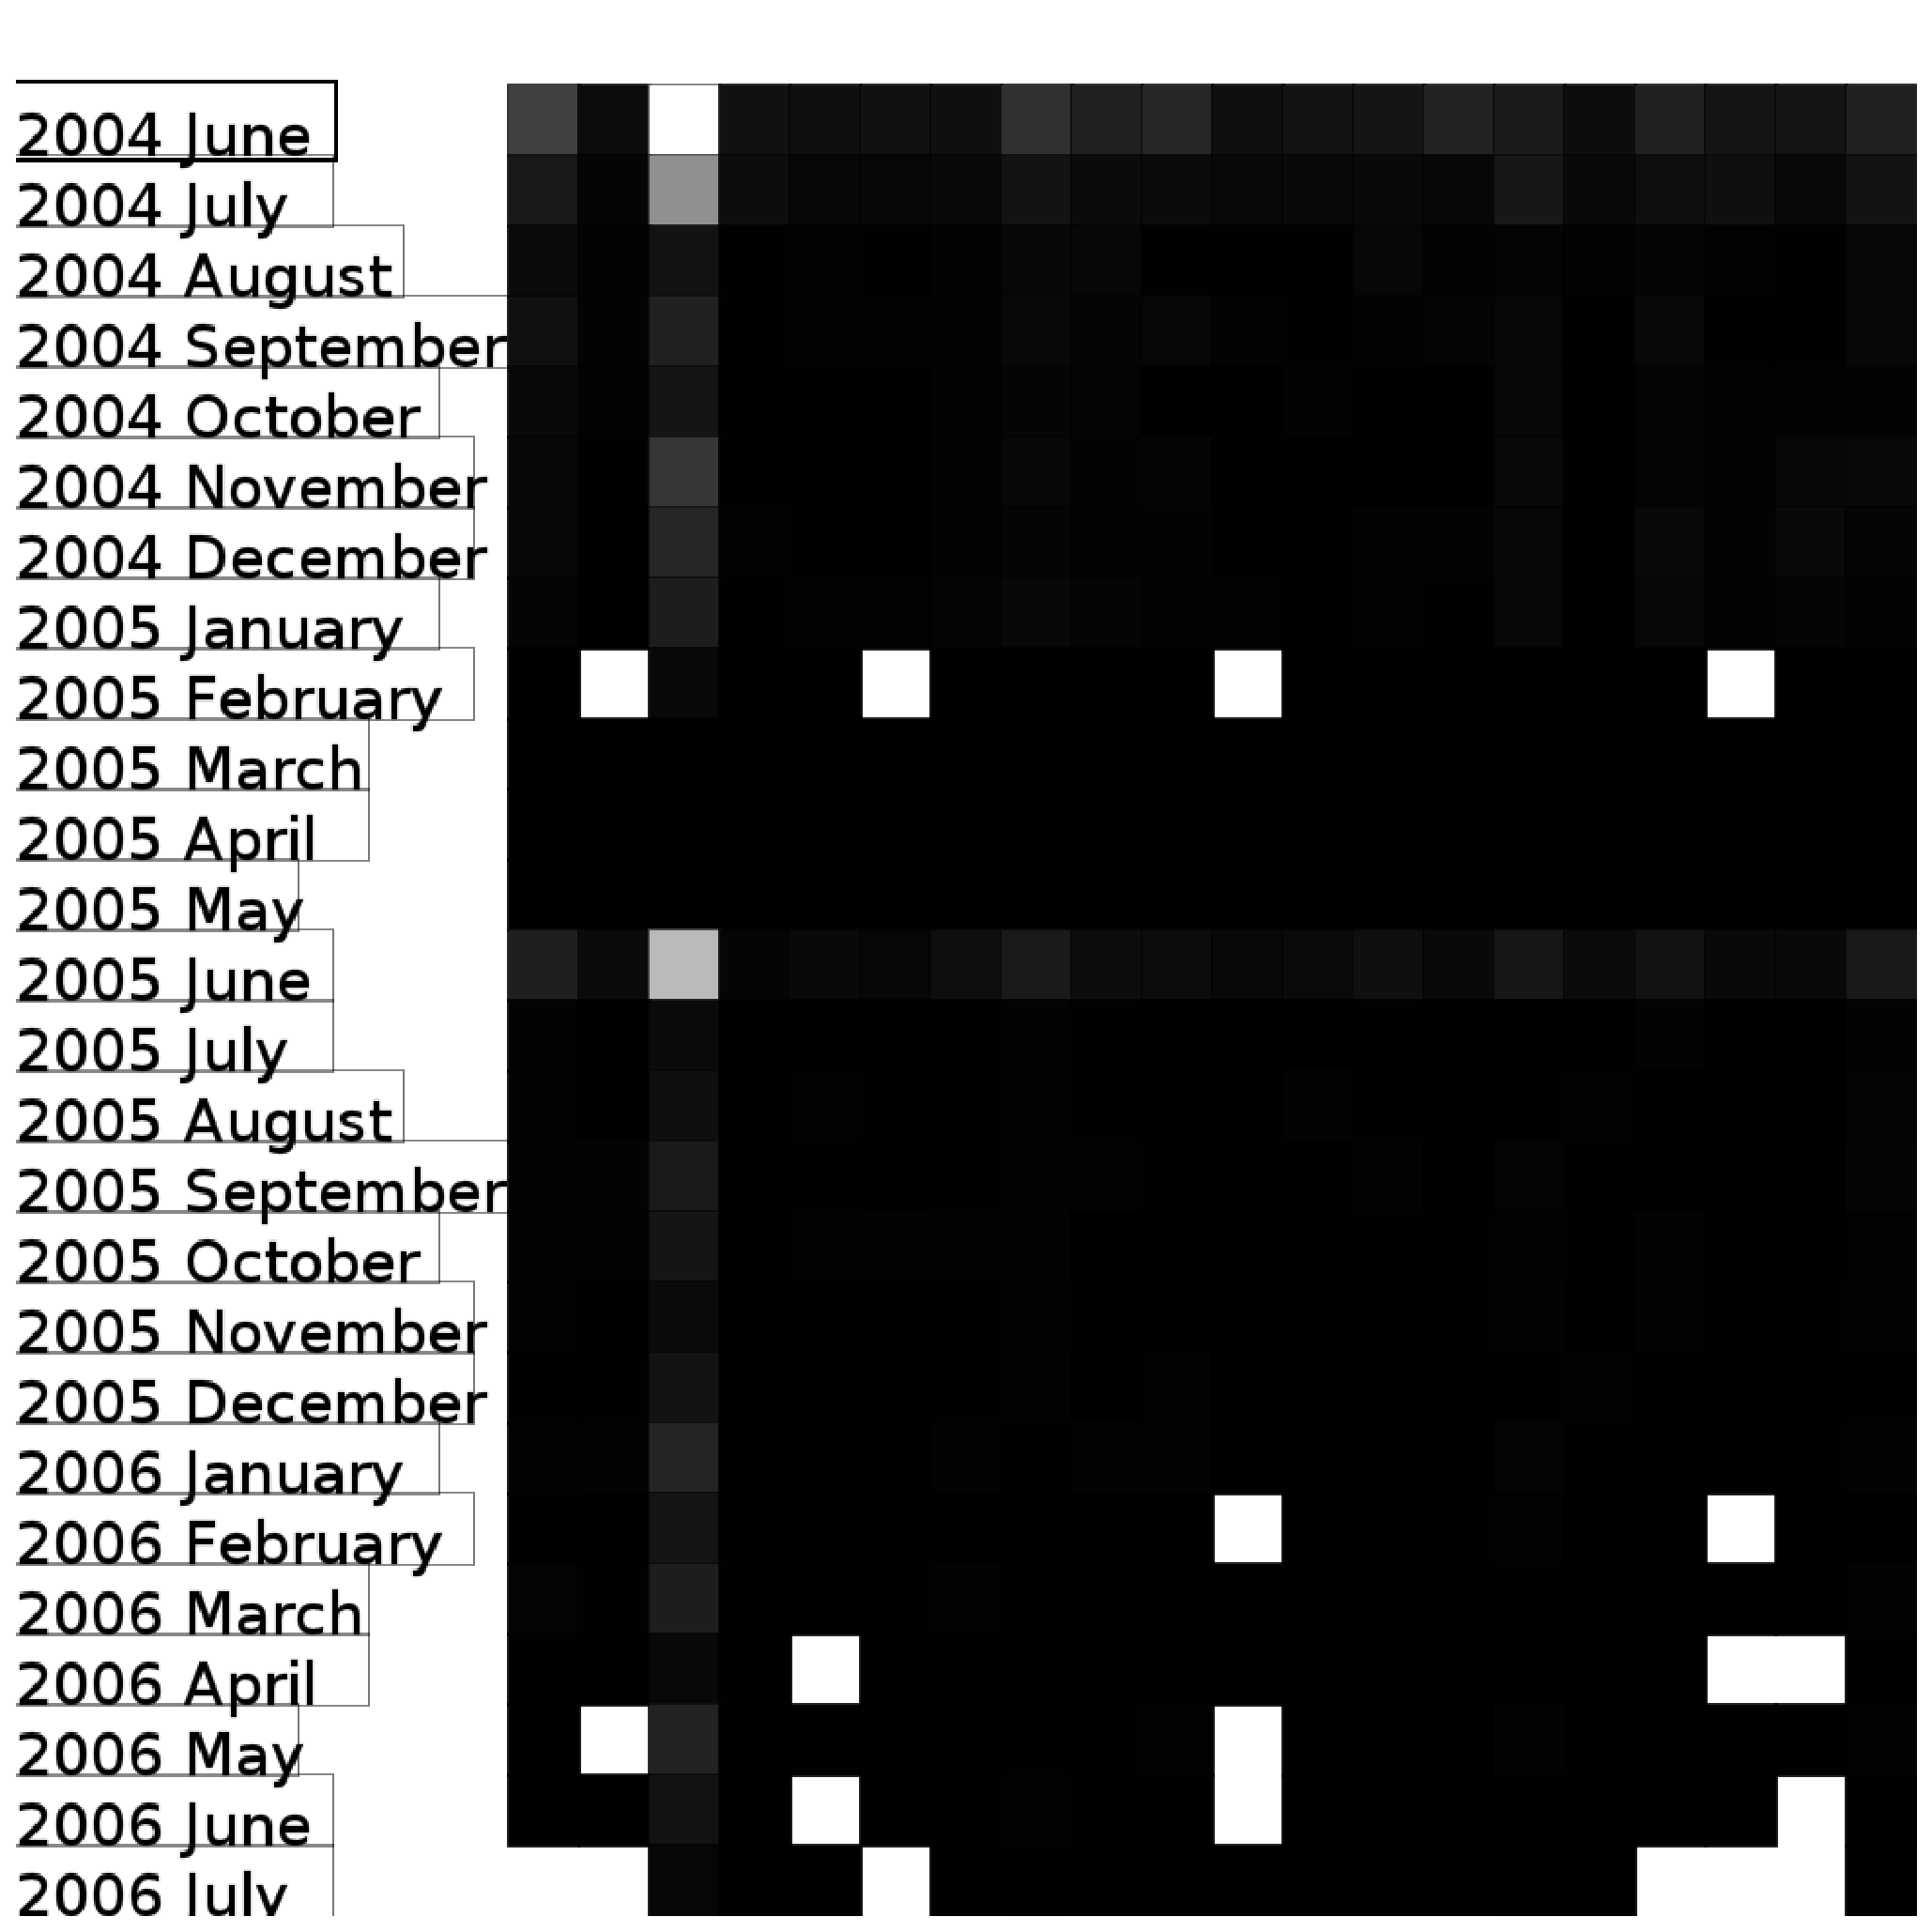
\includegraphics[width=0.45\textwidth]{maxdb7500-everything-by-month}
  \caption{MaxDB 7.500 Topics Analyzed with Static Topic Analysis, 20
    topics over the entire development history of MaxDB 7.500. Each
    box indicates the number of documents matching that topic in that
    month.}
  \label{fig:statictopics}
\end{figure}


\subsection{Validation}


%   1. well i'm stumped
%   2. look at it?
%   3. investigate those revisions and check the proportion etc
%   4. exploratory
%   5.   work it out
%8.   Validity Threats [0/5]
\section{Validity Threats}

In this study we are explicitly trusting that the programmers annotate
their changes with relevant information. We rely on the descriptions
they provide. If the language of checkin comments was automated we
would only be analyzing that.

We truncated the topics to top 10 tokens, this summary of a topic
might not have been as useful as determining the actual topic distance
between two word topic distributions. By truncating tokens we could be
losing valuable data.

Each project seemed to have their own kind of stop words, we did not
remove them, but perhaps dropping some of these stop words would aid
the clarity of such topic clusters, alternatively it might cause our
topic similarity plots to be fundamentally different. Perhaps our
methods of suggesting that topics are similar is not appropriate.

The number of commits per month is inconsistent some months have a lot
of changes where as some months have almost none.

%   1.   validation
%   2.   LDA is questionable
%   3.   blackbox problem
%   4.   not in the token
%   5.   multiple X token
%9.    Future Work

%10.   Conclusions




\section{Conclusions}
%11.   Start file file:/home/abez/projects/lda-paper/lda-paper.tex

Even with our liberal topic similarity metrics which produced both
long and short and trends we showed that there are only a few trends
in a repository which re-appear. Since so few trends re-appear and so
many trends appear only once this suggests that global topic analysis
might be ignoring local unique topics.


\subsection{ Future Work}

One avenue of future work we think is quite important is automatic
cluster labelling. Given a word distribution we should be able to
figure out a word or term which best describes that distribution
automatically.
Another avenue we wish to investigate the is value of applying
static community generated software taxonomies to the naming or
grouping of clusters




\bibliographystyle{latex8}
\bibliography{lda-paper}

%\bibliographystyle{abbrv}

\section{Appendix}

\begin{itemize}
\item We are missing a comparison of our technique to the classical technique
\end{itemize}

\end{document}
